\documentclass[a4paper,UKenglish]{lipics-v2016}
%This is a template for producing LIPIcs articles. 
%See lipics-manual.pdf for further information.
%for A4 paper format use option "a4paper", for US-letter use option "letterpaper"
%for british hyphenation rules use option "UKenglish", for american hyphenation rules use option "USenglish"
% for section-numbered lemmas etc., use "numberwithinsect"
 
\usepackage{microtype}%if unwanted, comment out or use option "draft"
\usepackage{pifont}
\usepackage{fp}
\usepackage{graphicx}
\usepackage{semantic}
\usepackage{lipsum}

\bibliographystyle{plainurl}% the recommended bibstyle

% ==================================================================================================

\title{Data exploration through dot-driven development\footnote{This 
  work was supported by Google Digital News Initiative.}}
\titlerunning{Data exploration through dot-driven development}

\author[1]{Tomas Petricek}
\affil[1]{The Alan Turing Institute, London, UK\\
  \texttt{tomas@tomasp.net}}
\authorrunning{T. Petricek}
\Copyright{Tomas Petricek}
\subjclass{D.3.2 Very high-level languages}
\keywords{Data science, type providers, pivot tables, aggregation}


\EventEditors{John Q. Open and Joan R. Acces}
\EventNoEds{2}
\EventLongTitle{42nd Conference on Very Important Topics (CVIT 2016)}
\EventShortTitle{CVIT 2016}
\EventAcronym{CVIT}
\EventYear{2016}
\EventDate{December 24--27, 2016}
\EventLocation{Little Whinging, United Kingdom}
\EventLogo{}
\SeriesVolume{42}
\ArticleNo{23}

% ==================================================================================================

\theoremstyle{plain}
\theoremstyle{definition}
\newtheorem{rmrk}{Remark}

% Formatting for source code & types
\definecolor{cmtclr}{rgb}{0.0,0.6,0.0}
\definecolor{kvdclr}{rgb}{0.0,0.0,0.6}
\definecolor{numclr}{rgb}{0.0,0.4,0.0}
\definecolor{strclr}{rgb}{0.4,0.3,0.0}
\definecolor{prepclr}{rgb}{0.6,0.0,0.2}

\newcommand{\vect}[1]{\langl #1 \rangl}
\newcommand{\langl}{\begin{picture}(4.5,7)
\put(1.1,2.5){\rotatebox{60}{\line(1,0){5.5}}}
\put(1.1,2.5){\rotatebox{300}{\line(1,0){5.5}}}
\end{picture}}
\newcommand{\rangl}{\begin{picture}(4.5,7)
\put(.9,2.5){\rotatebox{120}{\line(1,0){5.5}}}
\put(.9,2.5){\rotatebox{240}{\line(1,0){5.5}}}
\end{picture}}

\newcommand{\ball}[1]{\FPeval{\result}{clip(201+#1)}\textnormal{\ding{\result}}}

\newcommand{\lsep}{~\,|\,~}
\newcommand{\num}[1]{\textcolor{numclr}{#1}}
\newcommand{\str}[1]{\textnormal{\textcolor{strclr}{\sffamily "#1"}}}
\newcommand{\kvd}[1]{\textnormal{\textcolor{kvdclr}{\sffamily #1}}}
\newcommand{\ident}[1]{\textnormal{\sffamily #1}}
\newcommand{\qident}[1]{\textnormal{\sffamily \guillemotleft #1\guillemotright}}
% \newcommand{\qident}[1]{\textnormal{\sffamily ‹#1›}}

\newcommand{\dom}{\ident{dom}}

% ==================================================================================================

% TODO: Introduce pivot type provider somewhere early

\begin{document}
\maketitle

\begin{abstract}
Data literacy is becoming increasingly important in the modern world. While spreadsheets make 
simple data analytics accessible to a large number of people, creating transparent scripts that 
can be checked, modified, reproduced and formally analyzed requires expert programming skills. 
In this paper, we describe the design of a data exploration language that makes the task more 
accessible by embedding advanced programming concepts in a simple core language.

The core language uses type providers, but we employ them in a novel way -- rather than providing 
types with members for accessing data, we provide types with members that allow the user to access 
data, but also compose complex queries using only member access (``dot''). This lets us recreate 
functionality that usually requires complex type systems (row polymporphism, type state, 
dependent typing) in an extremely simple object-based language.

We formalize our approach using a minimal object-based calculus and prove that
programs constructed using the provided types represent valid data transformations. We then discuss 
a prototype implementation of the language, together with a simple editor that bridges
some of the gaps between programming and spreadsheets. We believe that this provides a pathway towards
democratizing data science -- our use of type providers significantly reduce the complexity of 
languages that one needs to understand in order to write scripts for exploring data.
\end{abstract}

% ==================================================================================================

\section{Introduction}
\label{sec:intro}

The rise of big data and open data initiatives means that there is an increasing amount of raw data 
available. At the same time, the fact that ``post-truth'' was chosen as the word of 2016 suggests 
that there has never been a greater need for increasing data literacy and building tools that let 
anyone -- including journalists and interested citizens -- explore such data and use it to support 
facts in a transparent way.

Spreadsheets made data exploration accessible to a large number of people, but operations 
performed on spreadsheets cannot be reproduced or replicated with different input parameters.
The manual mode of interaction is not repeatable and it breaks the link with the original data 
source, making spreadsheets error-prone [X]. The answer to this problem is to explore data 
programmatically. A program can be run repeatedly and its parameters can be modified.

However, even with the programming tools generally accepted as simple, exploring data is 
surprisingly difficult. For example, consider the following Python program (using the pandas
library), which reads a list of all Olympic medals ever awarded (see Appendix~\ref{app:olympics-csv}) 
and finds top 8 athletes by the number of gold medals they won in Rio 2016:

\noindent
\begin{equation*}
\begin{array}{l}
\ident{olympics} = \ident{pd.read\_csv}(\str{olympics.csv})\\[0.5em]
\ident{olympics}[\ident{olympics}[\str{Games}]==\str{Rio (2016)}]\\
\qquad .\ident{groupby}(\str{Athlete})\\
\qquad .\ident{agg}(\left\{\str{Gold}:\ident{sum}\right\})\\
\qquad .\ident{sort\_values}(\ident{by}=\str{Gold}, \ident{ascending}=\kvd{False})\\
\qquad .\ident{head}(\num{8})
\end{array}
\end{equation*}

\noindent
The code is short and easy to understand, but writing or modifying it requires the user to 
understand intricate details of Python and be well aware of the structure of the data source. 
The short example specifies operation parameters in three different ways -- indexing $[\ldots]$ 
is used for filtering; aggregation takes a dictionary $\left\{\ldots\right\}$ and sorting uses 
optional parameters. The dynamic nature of Python makes the code simple, but it also means that
auto-completion on member names (after typing dot) is not commonplace and so finding the operation
names (\ident{groupby}, \ident{sort\_values}, \ident{head}, ...) often requires using internet 
search. Furthermore, column names are specified as strings and so the user often needs to refer back
to the structure of the data source and be careful to avoid typos.

The language presented in this paper reduces the number of language features by making member access
the primary programming mechanism. Finding top 8 athletes by the number of gold medals from Rio 2016 
can be written as (in source code $\qident{\ldots}$ is written as \textquotesingle$\ldots$\textquotesingle):
%
\begin{equation*}
\begin{array}{l}
\ident{olympics}\\
\quad.\qident{filter data}.\qident{Games is}.\qident{Rio (2016)}.\ident{then}\\
\quad.\qident{group data}.\qident{by Athlete}.\qident{sum Gold}.\ident{then}\\
\quad.\qident{sort data}.\qident{by Gold descending}.\ident{then}\\
\quad.\qident{paging}.\ident{take}(\num{8})\\
\end{array}
\end{equation*}

\noindent
The language is object-based with nominal typing. This enables auto-completion that  
provides a list of available members when writing and modifying code. The members (such as 
\qident{by Gold descending}) are generated by a type provier based on the knowledge of
the data source and transformations applied so far -- thus only valid and meaningful 
operations are offered. The rest of the paper gives a detailed analysis and description of the mechanism.

\subparagraph{Contributions.} This paper explores an interesting particular corner of the 
programming language design space. We support it by a detailed analysis (Section~\ref{sec:analysis}), 
formal treatment (Section~\ref{sec:pivot}) and an implementation with 
a case study (Section~\ref{sec:impl}). Our contributions are:

\begin{itemize}
\item We use type providers in a new way (Section~\ref{sec:tps}). Previous work focused on providing 
  members for direct data access. In contrast, our pivot type provider (Section~\ref{sec:pivot}) lazily 
  provides types with members that can be used for composing queries, making it possible to perform
  entire date exploration through single programming mechanism (Section~\ref{sec:analysis-dot}).  

\item Our mechanism illustrates how to embed fancy types [X] into a simple nominally-typed programming  
  language (Section~\ref{sec:columns}). We track names and types of available columns of the 
  manipulated data set (using a mechanism akin to row types), but the same mechanism can be used for 
  embedding other advanced typing schemes into any Java-like language.
  
\item We implement the language (\url{github.com/the-gamma}), make it available as a JavaScript 
  component that can be used to build transparent data-driven visualizations (\url{thegamma.net}) 
  and discuss a case study visualizing fun facts about Olympic medals (Section~\ref{sec:impl}).

\item We formalize the language (Section~\ref{sec:foo}) and the type provider for data exploration
  (Section~\ref{sec:pivot}) and show that queries constructed using the type provider are valid
  (Section~\ref{sec:proofs}). Our formalization also covers the laziness of type providers, which
  is an important aspect not covered in the existing literature.
\end{itemize}

% ==================================================================================================

\section{Using type providers in a novel way}
\label{sec:tps}

The work presented in this paper consists of a simple nominally-typed host language and the pivot
type provider, which generates types with members that can be used to construct and execute queries
against an external data source. This section briefly reviews the existing work on type providers
and explains what is new about the pivot type provider.

\subparagraph{Information-rich programming.} Type providers were first presented as a mechanism
for providing type-safe access to rich information sources. A type provider is a compile-time 
component that imports external information source into a programming language [X]. It provides two 
things to the compiler or editor hosting it: a type signature that models the external source 
using structures understood by the host language (e.g.~types) and an implementation for the 
signatures which accesses data from the external source.

For example, the World Bank type provider [X] provides a fine-grained access to development 
indicators about countries. The following accesses CO2 emissions by~country~in~2010:
%
\begin{equation*}
\begin{array}{l}
\ident{world}.\ident{byYear}.\qident{2010}.\qident{Climate Change}.\qident{CO2 emissions (kt)}
\end{array}
\end{equation*}

\noindent
The provided schema consists of types with members such as \qident{CO2 emissions (kt)} and \qident{2010}.
The members are generated by the type provider based on the meta-data obtained from the World Bank.
The second part provided by the type provider is code that is executed when the above code is run.
For the example above, the code looks as follows:
%
\begin{equation*}
\begin{array}{l}
\ident{series.create}(\str{CO2 emissions (kt)},\str{Year},\str{Value},\\
\qquad \ident{world.getByYear}(\num{2010},\str{EN.ATM.CO2E.KT}))
\end{array}
\end{equation*}

\noindent
Here, a runtime library consists of a data series type (mapping from keys to values) and the 
\ident{getByYear} function that downloads data for a specified indicator represented by an ID. 
The type provider provides a type-safe access to known indicators, which exist only as strings in 
the compiled code, increasing safety and making data access easier thanks to auto-completion 
(which offers a list of available indicators).

\subparagraph{Types from data.} Recent work on the F\# Data library [X] uses type providers for 
accessing data in structured formats such as XML, CSV and JSON. This is done by inferring the 
structure of the data from a sample document, provided as a static parameter to a type provider.
In the following example, adapted from [X], a sample URL is passed to \ident{JsonProvider}:
%
\begin{equation*}
\begin{array}{l}
 \kvd{type}~\ident{Weather} = \ident{JsonProvider}\langl\str{http://api.owm.org/?q=London}\rangl \\[0.5em]
 \kvd{let}~\ident{ldn} = \ident{Weather.GetSample}()\\
 \ident{printfn}~\str{The temperature in London is \%f}~\ident{ldn.Main.Temp}
\end{array}
\end{equation*}

\noindent
As in the World Bank example, the JSON type provider generates types with members that let us access
data in the external data source -- here, we access the temperature using \ident{ldn.Main.Temp}. 
The provided code attempts to access the corresponding nested field and convert it to a number.
The relative safety property of the type provider guarantees that this will not fail if the sample 
is representative of the actual data loaded at runtime.
    
\subparagraph{Pivot type provider.} The pivot type provider presented in this paper follows the 
same general mechanism as the F\# type providers discussed above, although it is embedded in a 
simple language that runs in a web browser. 

The main difference between our work and the type providers discussed above is that we do not use
type providers for importing external data sources (by providing members that correspond to parts 
of the data). Instead, we use type providers for lazily generating types with members that let 
users compose type-safe queries over the data source. As discussed in Section~\ref{sec:foo}, we 
model the provided code by a relational algebra.

This means that our use of type providers is more akin to meta-programming or code generation with
one important difference -- the schema provided by the pivot type provider is potentially infinite
(as there are always more operations that can be applied). To support this, we use the fact that
type providers are integrated into the type system and types can be provided lazilly. This is 
also a new aspect of our formalization in Section~\ref{sec:foo}.

% ==================================================================================================

\section{Simplifying data scripting languages}
\label{sec:analysis}

In Section~\ref{sec:intro}, we contrasted a data exploration script written using a popular Python 
library pandas with a script written using the pivot type provider. In this section, we analyze 
what makes the Python code complex (Section~\ref{sec:analysis-why}) and how our design simplifies it.

\subsection{What makes data exploration scripts complex}
\label{sec:analysis-why}

We consider the Python example from Section~\ref{sec:intro} for concreteness, but the following 
four points are shared with other commonly used libraries and languages. We use them to guide our
alternative design discussed in the rest of this section.

\begin{itemize}
\item The filtering operation is written using indexing $[\ldots]$ while all other operations are
  written using member invocation with (optionally named) parameters. In the first case, we write
  an expression $\ident{olympics}[\str{Games}]==\str{Rio (2016)}$ returning a vector of Booleans
  while in the other, we specify a parameter value using $\ident{by}=\str{Gold}$. In other languges,
  a parameter can also be a lambda function specifying a predicate or a transformation.
  
\item The aggregation operation takes a dictionary $\left\{\ldots\right\}$, which is yet another
  concept the user needs to understand. Here, it lets us specify one or more aggregations to
  be applied over a group. A similar way of specifying multiple operations or results is common 
  in other languages. For example, anonymous types in LINQ play the same role.
      
\item The editor tooling available for Python is limited -- editors that provide auto-completion
  rely on a mix of advanced static analysis and simple (not always correct) hints and often fail
  for chained operations such as the one in our example\footnote{For an anecdotal evidence,
  see for example: \url{stackoverflow.com/questions/25801246/}}. Statically-typed languages
  provide better tooling, but at the cost of higher complexity\footnote{Again,
  See \url{fslab.org/Deedle}
  and \url{extremeoptimization.com/Documentation/Data_Frame/Data_Frames.aspx} }.

\item In the Python example (as well as in most other data manipulation 
  libraries\footnote{deedle, etc.}), column names are specified as strings. This makes static 
  checking of column names and auto-completion difficult. For example, \str{Gold} is a valid 
  column name when calling \ident{sort\_values}, but we only know that because it is a key of the 
  dictionary passed to \ident{agg} before.
\end{itemize}

\noindent
In our design, we unify many distinct languages constructs by making member
access the primary operation (Section~\ref{sec:analysis-dot}); we use simple nominal typing to
enable auto-completion (Section~\ref{sec:analysis-auto}); we use operation-chaining via member access
for constructing dictionaries (Section~\ref{sec:analysis-and}) and we track column names using the 
pivot type provider (Section~\ref{sec:columns}).

% --------------------------------------------------------------------------------------------------

\begin{figure}
\begin{center}
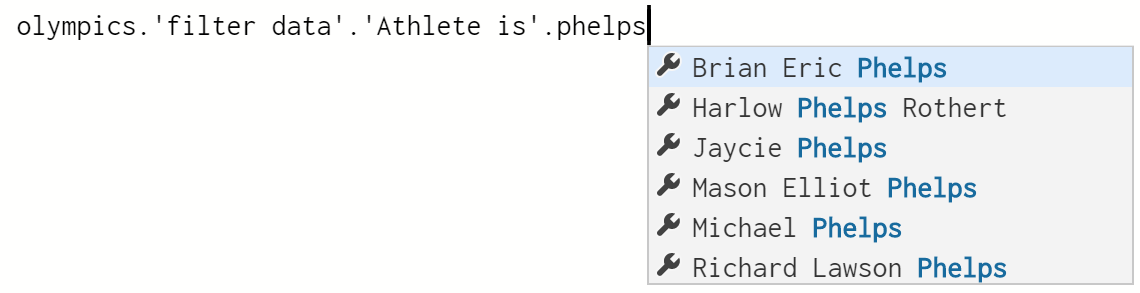
\includegraphics[scale=0.35,trim=0mm 0mm 0mm 0mm,clip]{filter.png} % left bottom right top
\end{center}
\caption{Auto-completion offering the available values of the athlete name column}
\label{fig:dot-driven}
\end{figure}

% --------------------------------------------------------------------------------------------------

\subsection{Unifying language constructs with member access}
\label{sec:analysis-dot}

LISP is perhaps the best example of a language that unifies many distinct constructs using a single
form. In LISP, everything is an s-experssion, that is, either a list or a symbol. In contrast, 
a typical data processing language uses a number of distinct constructs including indexers (for 
range selection and filtering), method calls (for transformations) and named parameters (for further 
configuration). Consider filtering and sorting:
%
\begin{equation*}
\begin{array}{l}
\ident{data}[\ident{data}[\str{Games}]==\str{Rio (2016)}] \qquad\ball{1}\\
\ident{data}.\ident{filter}(\kvd{fun}~\ident{row}\rightarrow\ident{row}.\ident{Games}==\str{Rio (2016)})\qquad\ball{2}\\
\ident{data}.\ident{sort\_values}(\ident{by}=\str{Gold}, \ident{ascending}=\kvd{False})\qquad\ball{3}\\
\end{array}
\end{equation*}

\noindent
Pandas uses indexers for filtering \ball{1} which can alternatively be written (e.g.~in 
LINQ) using a method taking a predicate as a lambda function \ball{2}. Operations that are 
parameterized only by column name, such as sorting in pandas \ball{3} are often methods with 
named parameters.

We aim to unify the above examples using a single language construct that offers a high-level programming
model\footnote{In contrast, s-expressions in LISP are typically used as a lower-level encoding of 
higher-level constructs. For example \ident{lambda} symbol encodes a lambda function as an s-expression.}
and can be supported by modern tooling (as discussed in Section~\ref{sec:analysis-auto}).
Member access provides an extremely simple programming construct that is, in conjunction with
the type provider mechanism capable of expressing the above data transformations in a uniform way: 
%
\begin{equation*}
\begin{array}{l}
\ident{data}.\qident{sort data}.\qident{by Gold descending}.\ident{then}\qquad\ball{1}\\
\ident{data}.\qident{filter data}.\qident{Games is}.\qident{Rio (2016)}.\ident{then}\qquad\ball{2}\\
\end{array}
\end{equation*}

\noindent
The member names tend to be longer and descriptive and we write them using \qident{...}.
The names are not usually typed by the user (see~Section~\ref{sec:analysis-auto}) and so the
length is not an issue when writing code. The above two examples illustrate two interesting
aspects of our approach. 

\subparagraph{Members, type providers, discoverability.}
When sorting \ball{1} the member that specifies how sorting is done includes the name of the
column. This is possible because the pivot type provider tracks the column names (see 
Section~\ref{sec:columns}) and provides members based on the available columns suitable
for use as sort keys. When filtering \ball{2}, the member \qident{Rio (2016)} is provided based
on the values in the data source (we discuss this furter in Section~\ref{sec:analysis-auto}).

These two examples illustrate that member access can be expressive, but it requires huge number
of types with huge number of members. Type providers address this by integration with the type
system (formalized in Section~\ref{sec:foo}) that discovers members lazily. This is why 
approaches based on code generation or pre-processors would not be viable.

Using descriptive member names is only viable when the names are discoverable. The above
code could be executed in a dynamically-typed languge that allows custom message-not-understood
handlers, but it would be impossible to get the name right when writing it. Our approach 
relies on discovering names through auto-completion as discussed in Section~\ref{sec:analysis-auto}.

\subparagraph{Expressivity of members.} 
Using member access as the primary mechanism for programming reduces the expressivity of the 
language -- our aim is to create a domain-specific language for data exploration, rather than
a general purpose language\footnote{Designing a general purpose language based on member access
is a separate interesting problem.}. For this purpose, the sequential nature of member accesses 
matches well with the sequential nature of data transformations.

The members provided, for example, for filtering limit the number of conditions that can be 
written, because the user is limited to choosing one of the provided members.
As discussed in the case study based on our implementation (Section~\ref{sec:impl}),
this appears sufficient for many common data exploration tasks. The mechanism could be made
more expressive, but we leave this for future work -- for example, the type provider could
accept or reject member names written by the user (as in internet search) rather than providing 
names from which the user can choose (as in web directories).

% --------------------------------------------------------------------------------------------------
 
\begin{figure}
\begin{equation*}
\quad \begin{array}{l}
\qident{drop columns}\\
\quad\rightarrow~\qident{drop Athlete}\\
\quad\rightarrow~\qident{drop Discipline}\\
\quad\rightarrow~\qident{drop Year}\\[0.5em]
\qident{sort data}\\
\quad\rightarrow~\qident{by Athlete}\\
\quad\rightarrow~\qident{by Athlete descending}\\
\quad\rightarrow~\qident{by Discipline}\\
\end{array}\qquad
\begin{array}{l}
\qident{group data}\\
\quad\rightarrow~\qident{by Athlete}\\
\qquad\quad\rightarrow~\qident{distinct Discipline}\\
\qquad\quad\rightarrow~\qident{average Year}\\
\qquad\quad\rightarrow~\qident{sum Year}\\[0.5em] 
\quad\rightarrow~\qident{by Year}\\
\qquad\quad\rightarrow~\qident{distinct Athlete}\\
\qquad\quad\rightarrow~\qident{distinct Discipline}\\
\end{array}
\end{equation*}
\caption{Subset of members provided by the pivot type provider}
\label{fig:pivot-members}
\end{figure}

% --------------------------------------------------------------------------------------------------
  
\subsection{Tooling and dot-driven development}
\label{sec:analysis-auto}

Source code editors for object-based languages with nominal type sytems often provide 
auto-completion for members of objects. This combination appear to work extremely well; the
member list is a complete list of what might follow after typing ``dot'' and it can be easily
obtained for an instance of known type. The fact that developers can often rely on just typing
``dot'' and choosing an appropriate member led to a semi-serious phrase dot-driven development,
that we (equally semi-seriously) adopt in this paper.

Type providers in F\# rely on dot-driven development when navigating through data. When writing code 
to access current temperature $\ident{ldn.Main.Temp}$ in Section~\ref{sec:tps}, the auto-completion
offers various available properties, such as \ident{Wind} and \ident{Clouds} once ``dot'' is typed
after $\ident{ldn.Main}$. Other type providers [X] follow a similar pattern. It is worth noting
that despite the use of nominal typing, the names of types rarely explicitly appear in code -- we
do not need to know the name of the type of $\ident{ldn.Main}$, but we need to know its members.
Thus the type name can be arbitrary [X] and is used more as a lookup key.

The pivot type provider presented in this paper uses dot-driven development for suggesting 
transformations as well as possible values of parameters. This is illustrated in Figure~\ref{fig:dot-driven}
where the user wants to obtain medals of a specific athlete and is offered a list of possible 
names. The editor filters the list as the user starts typing the required name. 

In Figure~\ref{fig:pivot-members}, we list a subset of the provided members that were used in the
example in Section~\ref{sec:intro}. After choosing \qident{sort data}, the user is offered 
the possible sorting keys and directions. After choosing \qident{group data}, the user first 
selects the grouping key and then can choose one or more aggregations that can be applied on
other columns of the group. Thus an enitre data transformation (such as choosing top 8 athletes
by the number of gold medals) can be constructed using dot-driven development.
  
\subparagraph{Values vs. types.}
As the Figure~\ref{fig:dot-driven} illustrates, the pivot type provider sometimes blurs the 
distinction between values and (members of) types. In the example in Section~\ref{sec:intro},
\str{Rio (2016)} is a string value in Python, but a statically-typed member \qident{Rio (2016)}
when using pivot type provider. This is a recurring theme in type provider development\footnote{The
\ident{Individuals} property in the Freebase type provider [X] imports values into types in a similar way.}.

Our language supports method calls such as $\ident{head}(\num{8})$ and an alternative design for
filtering would be to provide a method such as $\qident{Games is}(\str{Rio (2016)})$. However,
the fact that we can offer possible values largely simplifies writing of the script for the most 
common case when the user is interested in one of the known values.

Unlike in traditional development, a data scientist doing data exploration often has the entire 
data set available. The pivot type provider uses this when offering possible values for filtering
(Section~X), but all other operations (Section~Y) require only meta-data (names and types of 
columns). Following the example of type providers for structured data formats [X], the schema could
be inferred from a representative sample.

% --------------------------------------------------------------------------------------------------
   
\subsection{Expressing structured logic using members}
\label{sec:analysis-and}

In the motivating example, the \ident{agg} method takes a dictionary that specifies one or more 
aggregates to be calculated over a group. We sum the number of gold medals, but we could also sum
the number of silver and bronze medals, concatenate names of teams for the athlete and perform other 
aggregations. In this case, we provide a nested structure (list of aggregations) as a parameter of 
a single operation (grouping). 

This is an interesting case, because when encoding program as a sequence of member accesses, 
there is no built-in support for nesting. In the pivot type provider, we use ``then'' design
pattern to provide operations that require nesting. The following example specifies multiple 
aggregations and then sorts data by multiple keys:
%
\begin{equation*}
\begin{array}{l}
\ident{olympics}.\\
\quad\qident{group data}.\qident{by Athlete}.\\
\qquad.\qident{sum Gold}.\qident{sum Silver}.\qident{concat Team}.\ident{then} \qquad\ball{1}\\
\quad.\qident{sort data}.\\
\qquad.\qident{by Gold descending}.\qident{and Silver descending}.\ident{then} \qquad\ball{2}\\
\end{array}
\end{equation*}

\noindent
When grouping, we sum the number of gold and silver medals and concatenates team names~\ball{1}. 
Then we sorts the grouped data using multiple sorting keys \ball{2} -- first by number of gold 
medals and then by silver medals (within a group with the same number of gold medals). 

\subparagraph{The ``then'' pattern.}
Nesting is no doubt essential programming construct and it may very well be desirable to support it 
directly in the language, but the ``then'' pattern lets us express it without explicit langauge
support. In both cases, the nested structure is specified by selecting one or more members and then 
ending the nested structure using the \ident{then} member.

In case of grouping, we choose aggregations (\qident{sum Gold}, \qident{concat Team}, etc.) after 
we specify grouping key using \qident{by Athlete}. In case of sorting, we specify the first key
using \qident{by Gold descending} and then add more nested keys using \qident{and Silver descending}.
Thanks to the dot-driven development and the ``then'' pattern, the user is offered possible 
parameter values (aggregations or sorting keys) even when creating a nested structure. This is
harder to do with general-purpose nesting as ordinary languages (even domain-specific languages)
often provide many different ways for creating a nested structure.

\subparagraph{Renaming columns.}
The pivot type provider automatically chooses names for the columns obtained as the result of
aggregation. In the above example \ball{1}, the resulting data set will have columns Athlete
(the grouping key) together with Gold, Silver and Team (based on the aggregated columns).
The user cannot currently rename the columns.

% https://github.com/fsharp/fslang-design/blob/master/FSharp-4.0/StaticMethodArgumentsDesignAndSpec.md

In F\# type providers, this could be done using methods with static parameters [X] by writing, 
for example, $\ident{g}.\qident{sum Gold as}\langl\str{Total Gold}\rangl()$. In F\#, the value of 
the static parameter (here, \str{Total Gold}) is passed to the type provider, which can use it to
generate the type signature of the method and the return type with member name according to the
value of the static parameter.

% ==================================================================================================

\section{Tracking column names}
\label{sec:columns}

The last difficulty with data scripting discussed in Section~\ref{sec:analysis-why} is that pandas 
(and other data exploration libraries, even for statically-typed languages) track column names as 
strings at runtime, making code error-prone and auto-complete on column names difficult to provie.
Proponents of static typing would correctly point out that column names and their types can be
tracked by a more sophisticated type system. 

In this section, we discuss our approach -- we track column names statically using a mechanism
that is inspired by row types and type state (Section~\ref{sec:columns-row}), however we 
embed the mechanism using type providers into a simple nominal type system (Section~\ref{sec:columns-tp}).
This way, the host language for the pivot type provider can be extremely simple -- and indeed, the
mechanism could be added to languages such as Java or TypeScript with minimal effort. 

% --------------------------------------------------------------------------------------------------

\begin{figure}

\begin{equation*}
\inference[(\emph{drop-start})~]
  {\Gamma \vdash e : [f_1\!:\!\tau_1, \ldots, f_n\!:\!\tau_n]}
  {\Gamma \vdash e.\qident{drop columns}: [f_1\!:\!\tau_1, \ldots, f_n\!:\!\tau_n]_{\ident{drop}}}
\end{equation*}

\begin{equation*}
\inference[(\emph{drop-col})~]
  {\Gamma \vdash e : [f_1\!:\!\tau_1, \ldots, f_n\!:\!\tau_n]_{\ident{drop}}}
  {\Gamma \vdash e.\qident{drop~$f_i$}: [f_1\!:\!\tau_1, \ldots, f_{i-1}\!:\!\tau_{i-1}, f_{i+1}\!:\!\tau_{i+1}, \ldots, f_n\!:\!\tau_n ]_{\ident{drop}}}
\end{equation*}

\begin{equation*}
\inference[(\emph{drop-then})~]
  {\Gamma \vdash e : [f_1\!:\!\tau_1, \ldots, f_n\!:\!\tau_n]_{\ident{drop}}}
  {\Gamma \vdash e.\qident{then}: [f_1\!:\!\tau_1, \ldots, f_n\!:\!\tau_n]}
\end{equation*}


\caption{Tracking available column names with row types and type state}
\label{fig:fancy-types}
\end{figure}

% --------------------------------------------------------------------------------------------------

\subsection{Using row types and type state}
\label{sec:columns-row}

There are several common data transformations that modify the structure of the data set and affect
what columns (and of what types) are available. When grouping and aggregating data, the resulting
data set has columns depending on the aggregates calculated. Another simpler operation is adding
or removing a column from the data set. For example, given the Olympic medals data set, we can 
drop games and year as follows:
%
\begin{equation*}
  \begin{array}{l}
    \ident{olympics}.\qident{drop columns}.\qident{drop Games}.\qident{drop Year}.\ident{then}
  \end{array}
\end{equation*}

\noindent
Operations on the type of rows in the data set can be captured using row types [X]. In addition, 
we need to annotate type with a form of type state [Y] to restrict what operations are available. 
When dropping columns, we first access the \qident{drop columns} member, which sets the state to
a state where we can drop individual columns using \qident{drop $f$}. The \ident{then} member can 
then be used to complete the operation and choose another transformation.

To illustrate tracking of columns using row types and type state, consider a simple language with
variables (representing external data sources) and member access. Types can be either primitive 
types $\alpha$, types annotated with a type state \ident{lbl} or row type with fields $f$:
%
\begin{equation*}
\begin{array}{rcl}  
e&=&v \lsep e.N\\
\tau&=&\alpha \lsep \tau_\ident{lbl} \lsep [f_1\!:\!\tau_1, \ldots, f_n\!:\!\tau_n] 
\end{array}  
\end{equation*}

\noindent
Typing rules for members that are used to drop columns are shown in Figure~\ref{fig:fancy-types}.
When \qident{drop columns} is invoked on a record, the type is annotated with a state \ident{drop}
(\emph{drop-start}) indicating that individual columns may be dropped. The \ident{then} 
operation (\emph{drop-then}) removes the state label. Individual members can be removed using
\qident{drop $f_i$} and the (\emph{drop-col}) rule ensures the dropped column is available in the
input row type and removes it.

Other data transformations could be type checked in a similar way, but there are two drawbacks.
First, row types and type state (although relatively straightforward) make the host language more
complex. Second, rules such as (\emph{drop-col}) make auto-completion more difficult, because the
editor needs to understand the rules and calculate what members may be invoked. This is a distinct
operation from type checking and type infernece (which operate on complete programs) that needs 
to be formalized and implemented.

% --------------------------------------------------------------------------------------------------

\subsection{Using the pivot type provider}
\label{sec:columns-tp}

In our approach, the information about available fields is used by a type provider to provide
types with appropriate members. This is hidden from the host language, which only sees class types
with members. Provided class definitions consist of a constructor and members: 
%
\begin{equation*}
\begin{array}{rcl}
 l &=& \kvd{type}~C(x:\tau) = \overline{m} \\
 m &=& \kvd{member}~N:\tau= e
\end{array}
\end{equation*}

\noindent
During type-checking, the type system keeps track of a list of provided class definitions $L$. 
Checking member access is then just a matter of finding the corresponding class definition and
finding the member type:
%
\begin{equation*}
\inference[(\emph{member})~]
  {L; \Gamma \vdash e : C & \kvd{type}~C(x:\tau) = ..\;\kvd{member}~N_i : \tau_i = e_i\;.. \in L}
  {L; \Gamma \vdash e.N_i:\tau_i}
\end{equation*}

\noindent
The rule, adapted from [X], does not capture laziness of type providers that is 
important for the pivot type provider (where the number of provided classes is potentially 
infinite). We discuss this aspect in Section~\ref{sec:foo}.

Using type providers and nominal type system seemingly hides knowledge about fields available
in the data set. However, for types constructed by the pivot type provider, we can define a 
mapping \ident{fields} that returns the fields available in the data set represented by the 
class. The type provider encodes the logic expressed in Section~\ref{sec:columns-row} in the
following sense:

\begin{rmrk}[Encoding of fancy types]
\label{thm:encoding-fancy}
If $\Gamma\vdash e:[f_1\!:\!\tau_1, \ldots, f_n\!:\!\tau_n]$ using a type system defined in 
Figure~\ref{fig:fancy-types} and $\Gamma\vdash e:C$ using nominal typing and $C$ is a type 
provided by the pivot type provider then $\ident{fields}(C) = \{ f_1\mapsto\tau_1, \ldots, f_n\mapsto\tau_n \}$.
\end{rmrk}

\noindent
In the following two sections, we focus on formalizing the pivot type provider and the nominally 
typed host language. We define the \ident{fields} predicate in Section~\ref{sec:proofs} and use it 
to prove properties of the pivot type provider.

We do not fully develop the type system based on fancy types sketched in Section~\ref{sec:columns-row}.
However, the remark illustrates one interesting aspect of our work -- the type provider 
mechanism makes it possible to express safety guarantees that would normally require row types and 
type state in a simple nominally typed language. In a similar way, type providers have been used
to encode session types [X], suggesting that this is a generally useful approach.

% ==================================================================================================

\begin{figure}

\begin{equation*}
\begin{array}{rclll}
  D & = & \multicolumn{3}{l}{ 
    \{f_1\mapsto \vect{v_{1,1},\ldots,v_{1,r}}, \ldots, f_n\mapsto \vect{v_{n,1},\ldots,v_{n,r}}\} 
  }\\[0.5em]
  e & = & \Pi_{f_1, \ldots, f_n} (e) &&\textnormal{Projection -- select specified column names}\\
   & \lsep & \sigma_\varphi (e) &&\textnormal{Selection -- filter rows by given predicate}\\
   & \lsep & \tau_{f_1\mapsto\omega_1, \ldots, f_n\mapsto\omega_n}(e) &&\textnormal{Sorting -- sort by specified columns}\\
   & \lsep & \Phi_{f, \rho_1/f_1, \ldots, \rho_n/f_n} (e) &&\textnormal{Grouping -- group by and calculate aggregates}
   \\[0.5em]
  \omega & = & \ident{desc}\lsep\ident{asc}  &&\textnormal{Sort order -- descending or ascending}\\
  \rho & = & \ident{count}  &&\textnormal{Count number of rows in the group}\\
   & \lsep & \ident{sum}~f  &&\textnormal{Sum numerical values of the column $f$}\\
   & \lsep & \ident{dist}~f &&\textnormal{Count number of distinct values of the column $f$}\\
   & \lsep & \ident{conc}~f &&\textnormal{Concatenat string values of the column $f$}\\
\\
\end{array} 
\end{equation*}

\vspace{-1.5em}
\caption{Relational algebra with values, sorting and aggregation}
\label{fig:foo-rel}
\end{figure}

% --------------------------------------------------------------------------------------------------

\begin{figure}
\begin{equation*}
\begin{array}{l}
\Pi_{f_{p(1)}, \ldots, f_{p(m)}} \{f_1\mapsto \vect{v_{1,1},\ldots,v_{1,r}}, \ldots, f_n\mapsto \vect{v_{n,1},\ldots,v_{n,r}}\} \leadsto \\
  \quad \{f_{p(1)}\mapsto \vect{v_{p(1),1},\ldots,v_{p(1),r}}, \ldots, f_{p(m)}\mapsto \vect{v_{p(m),1},\ldots,v_{p(m),r}}\}  
\\
\\
\sigma_\varphi \{f_1\mapsto \vect{v_{1,1},\ldots,v_{1,r}}, \ldots, f_n\mapsto \vect{v_{n,1},\ldots,v_{n,r}}\} \leadsto\\
  \quad \{f_1\mapsto \vect{\ldots, v_{1,j}, \ldots}, \ldots, f_n\mapsto \vect{\ldots, v_{n,j},\ldots}\}
  \qquad (\forall j.\;\varphi\, \{f_1\mapsto v_{1,j}, \ldots, f_n\mapsto v_{n,j}\})
\\
\\
\tau_{f_{p(1)}\mapsto\omega_1, \ldots, f_{p(m)}\mapsto\omega_m} \{f_1\mapsto \vect{v_{1,1},\ldots,v_{1,r}}, \ldots, f_n\mapsto \vect{v_{n,1},\ldots,v_{n,r}}\} \leadsto\\
  \quad \{f_1\mapsto \vect{v_{1,q(1)},\ldots,v_{1,q(r)}}, \ldots, f_n\mapsto \vect{v_{n,q(1)},\ldots,v_{n,q(r)}}\} 
  \quad \textnormal{where $q$ permutation}\\
  \qquad \textnormal{such that}~\forall i, j.~i\leq j\implies(u_{1,i}, \ldots, v_{m,i}) \leq (v_{1,j}, \ldots, v_{m,j})~ \textnormal{where}\\
  \qquad \quad u_{k,l}=v_{p(k),q(l)} \quad \,~~(\textnormal{when}~\omega_k=\ident{asc}) \\
  \qquad \quad u_{k,l}=-v_{p(k),q(l)} \quad (\textnormal{when}~\omega_k=\ident{desc})
  \\
  \\
\Phi_{f_i, \rho_1/f_1', \ldots, \rho_m/f_m'} \{f_1\mapsto \vect{v_{1,1},\ldots,v_{1,r}}, \ldots, f_n\mapsto \vect{v_{n,1},\ldots,v_{n,r}}\} \leadsto\\
  \quad \{f_1' \mapsto a_1, \ldots, f_m'\mapsto a_m, f_i\mapsto b \} 
  \quad \textnormal{where}\\
  \qquad \{g_1,\ldots,g_s\}=\{\{l~|~k\in 1\ldots r, ~v_{i,l}=v_{i,k}\}, ~l\in 1\ldots r\} \\
  ~~\begin{array}{ll}    
    \qquad b = \vect{v_{i,k_1},\ldots,v_{i, k_s}} & \textnormal{where}~k_j \in g_j \\
    \qquad a_i = \vect{|g_1|, \ldots, |g_s|}  & \textnormal{when}~\rho_i = \ident{count} \\
    \qquad a_i = \vect{\Sigma_{k\in g_1}v_{j,k}, \ldots, \Sigma_{k\in g_s}v_{j,k}} & \textnormal{when}~\rho_i = \ident{sum}~f_j \\
    \qquad a_i = \vect{\Pi_{k\in g_1}v_{j,k}, \ldots, \Sigma_{k\in g_s}v_{j,k}}   & \textnormal{when}~\rho_i = \ident{conc}~f_j \\
    \qquad a_i = \vect{|\{v_{j,k}\,|\, k\in g_1\}|, \ldots, |\{v_{j,k}\,|\, k\in g_s\}|}  & \textnormal{when}~\rho_i = \ident{dist}~f_j \\
  \end{array}\\
\end{array}
\end{equation*}

\caption{Vector-based semantics for operations of the extended relational algebra}
\label{fig:foo-relsem}
\end{figure}

% --------------------------------------------------------------------------------------------------

\section{Formalising the host language and runtime}
\label{sec:foo}

Type providers often provide a thin type-safe layer over richer untyped runtime components. In case 
of providers for data access (Section~\ref{sec:tps}), the untyped runtime component performs operations
over external data sources. In case of the pivot type provider, the untyped runtime component 
is a relational algebra modelling data transformations. We formalize the relational algebra in 
Section~\ref{sec:foo-rel}, together with the object-based host language in Section~\ref{sec:foo-foo}.

\subsection{Relational algebra with vector semantics}
\label{sec:foo-rel}

The focus of our work is on data aggregation and so we use a form of relational algebra with 
extensions for grouping and sorting [X,Y,Z]. The syntax is defined in Figure~\ref{fig:foo-rel}.
We write $f$ for column (field) names and we include definition of a data value $D$, which maps
columns to vectors of length $r$ storing the data (values $v$ are defined below).
Aside from standard projection $\Pi$ and selection $\sigma$, our algebra includes sorting 
$\tau$ which takes one or more columns forming the sort key (with sort order $\omega$)
and aggregation $\Phi$, which requires a single grouping key and several aggregations together with 
names of the new columns to be returned.

The semantics of the algbra is given in Figure~\ref{fig:foo-relsem}. We use vector-based semantics
to support sorting and duplicate entries, but otherwise the formalization captures the usual
behaviour. In projection and sorting, we write $f_{p(1)}, \ldots, f_{p(m)}$ to refer to a selection
of fields from $f_1, \ldots, f_n$. Assuming $m\leq n$, $p$ can be seen as a mapping from $\{1\ldots m\}$
to a subset of $\{1\ldots n\}$. In selection, $\varphi$ is a predicate applied to a mapping from 
column names to values. In sorting, we assume that there is a permutation on row indices $q$ such
that the tuples obtained by selecting values according to the given sort key are ordered. The 
auxiliary definition $u_{k,l}$ negates the number to reverse the sort order when descending order
is required.

The most complex operation is grouping. We need to group data by the value of the column $f_i$ and
then apply aggregations $\rho_1,\ldots,\rho_m$. To do this, we first obtain a set of groups $g_1,\ldots, g_s$
where each group represents a set of indicies of rows belonging to each group. For a given group 
$g_i$ we can then obtain values of column $j$ for rows in the group as $\{v_{j,k}\,|\, k\in g_i\}$.
This is used to calculate the resulting data set -- the field $f_i$ becomes a new column formed
by the group keys (obtained by picking one of the indices from $g_j$ for each group); other fields
are calculated by aggregating data in various ways -- $|g_i|$ gives the number of rows in the group,
$\Sigma$ sums numerical values and $\Pi$ (a slight notation abuse) concatenates string values. 

% --------------------------------------------------------------------------------------------------

\begin{figure}
\begin{equation*}
\begin{array}{rcl}
  v &=& C(v)\,\, \lsep \ident{series}\langl \tau_1, \tau_2 \rangl(v)\; \lsep n \lsep s \lsep D \\
  e &=& C(e)\,\, \lsep \ident{series}\langl \tau_1, \tau_2 \rangl(e)\;\, \lsep x \lsep v \lsep e.N \lsep \ldots\\
  E &=& C(E) \lsep \ident{series}\langl \tau_1, \tau_2 \rangl(E)\, \lsep E.N \\
    &|& \Pi_{f_1, \ldots, f_n}(E) \lsep \sigma_\varphi(E) \lsep \tau_{f_1, \ldots, f_n}(E) \lsep \Phi_{f_i, \rho_1/f_1', \ldots, \rho_m/f_m'} (E) \\
    \\
 \tau &=& C \lsep \kvd{num} \lsep \kvd{string} \lsep \ident{series}\langl \tau_1, \tau_2 \rangl \lsep \ident{Query}\\
 l &=& \kvd{type}~C(x:\tau) = \overline{m} \\
 m &=& \kvd{member}~N:\tau= e
\end{array}
\end{equation*}
\vspace{-1em}

\[
\inference[(\emph{member})~]
{ L(C) = (\kvd{type}~C(x:\tau)= \ldots~\kvd{member}~N_i : \tau_i = e_i~\ldots), L'}
{ (C(v)).N_i \leadsto_L e_i[x \leftarrow v] }\\
\]
\vspace{-2.5em}

\[
\inference[(\emph{context})~]
{e \leadsto_L e'}
{E[e] \leadsto_L E[e']}
\]

\caption{Syntax and remaining reduction rules of the Foo calculus}
\label{fig:foo-syntax}
\end{figure}

% --------------------------------------------------------------------------------------------------

\subsection{Foo calculus with lazy context}
\label{sec:foo-foo}

We model the host language using a variant of the Foo calculus [X]. The core of the calculus models
a simple object-based language with objects and members. The syntax of the language is shown in
Figure~\ref{fig:foo-syntax}. The relational algebra defined in Figure~\ref{fig:foo-rel} is included
in the Foo calculus as a model of the runtime components of the pivot type provider -- the values
include the data value $D$ and the expressions include all the operations of the relational algebra.

The Foo calculus includes two special types. \ident{Query} is a type of data and queries 
constructed using the relational algebra. The type $\ident{series}\langl \tau_1, \tau_2 \rangl$ 
models a data series mapping keys of type $\tau_1$ to values of type $\tau_2$. A series is created 
as a result of a query written using the pivot type provider. In the actual implementation, a series 
can be passed to a charting library. A series is a statically-typed wrapper over a \ident{Query} 
value and the proofs in Section~\ref{sec:proofs} show that a series obtained from the pivot type 
provider contains keys and values of matching types.

\subparagraph{Reduction rules.} The reduction relation $\leadsto_L$ is prameterized by a function
$L$ that maps class names to class definitions, together with nested classes associated with the
class definition (used during type-checking as discussed below). The map is not used in the 
reduction rules for the relational algebra, given in Figure~\ref{fig:foo-relsem} and so it was 
omitted there.

The remaining reduction rules are given in Figure~\ref{fig:foo-syntax}. The (\emph{member}) rule 
performs lookup using $L(C)$ to find the definition of the member that is being accessed and then
it reduces member access by substituting the evaluated constructor argument $v$ for a variable $x$.
We assume standard capture-avoiding substitution $[x\leftarrow v]$. The rule ignores the nested 
class definitions $L'$. The (\emph{context}) rule performs reduction in an evaluation context $E$.

\subparagraph{Type checking.} One interesting aspect of type-checking with type providers is that
type providers can provide potentially infinite number of types. In F\#, the types are provided 
lazily as the type checker explores parts of the type space used by the program [X]. Consider:
%
\begin{equation*}
\ident{olympics}.\qident{group data}.\qident{by Athlete}.\qident{sum Gold}.\ident{then}
\end{equation*}

\noindent
The type checker initially knows the type of $\ident{olympics}$ is a class $C_1$ with member 
$\qident{group data}$ and it knows that the type of this member is $C_2$. However, it only needs to 
obtain full definition of $C_2$ when checking the member $\qident{by Athlete}$. Types of other 
member of $C_1$ remain unevaluated when they do not appear in the source code. This aspect of type
providers have been omitted in previous work [X,Y], but it is necessary for the pivot type provider.
The typing rules given are written using the following judgement:
%
\begin{equation*}
L_1; \Gamma \vdash e : \tau; L_2
\end{equation*}

\noindent
The judgement states that given class definitions $L_1$ and a variable context $\Gamma$, the type
of expression $e$ is $\tau$ and the type checking evaluated further class definitions that are
now included in $L_2$. The structure of class definitions $L_1$ is a function mapping a class name 
$C$ to a pair consisting of the definition and a function that provides definitions of 
further classes: 
%
\begin{equation*}
L_1(C) = \kvd{type}~C(x:\tau) = \overline{m}, L'
\end{equation*}

\noindent
The types of members of the class $C$ may be already known classes defined by $L_1$, but also classes 
defined by $L'$. This models laziness as $L'$ is a function that may never be evaluated. 

The rules that define type-checking are shown in Figure~\ref{fig:foo-typecheck}. The two rules
that force the discovery of new classes are (\emph{new}) and (\emph{member}). In both cases,
we perform a lookup using $L_2(C)$ which returns a class definition together with further classes
$L$. We treat functions as sets and join $L_2$ with further classes defined by $L$ using $L_2 \cup L$.

% --------------------------------------------------------------------------------------------------

\begin{figure}[t]

\[
\inference[(\emph{num})~]{}{L; \Gamma \vdash n : \kvd{num}; L }
\quad
\inference[(\emph{string})~]{}{L; \Gamma \vdash s : \kvd{string}; L}
\quad
\inference[(\emph{var})~]{}{L; \Gamma, x:\tau\vdash x:\tau; L}
\]
\vspace{-2em}

\[
\inference[(\emph{data})~]
  {L; \Gamma \vdash v_{i,j} : \tau;L \quad \tau \in \{ \kvd{num}, \kvd{string} \}}
  {L; \Gamma \vdash \{f_1\mapsto \vect{v_{1,1},\ldots,v_{1,r}}, \ldots, f_n\mapsto \vect{v_{n,1},\ldots,v_{n,r}}\} : \ident{Query};L }
\]
\vspace{-2em}

\[
\inference[(\emph{proj})~]
  {L_1; \Gamma\vdash e : \ident{Query}; L_2}
  {L_1; \Gamma\vdash \Pi_{f_1, \ldots, f_n} (e) : \ident{Query}; L_2}
\qquad\inference[(\emph{sort})~]
  {L_1; \Gamma\vdash e : \ident{Query}; L_2}
  {L_1; \Gamma\vdash \tau_{f_1, \ldots, f_n}(e): \ident{Query}; L_2}
\]

\[
\inference[(\emph{sel})~]
  {L_1; \Gamma\vdash e : \ident{Query}; L_2}
  {L_1; \Gamma\vdash \sigma_\varphi (e) : \ident{Query}; L_2}
\qquad
\inference[(\emph{group})~]
  {L_1; \Gamma\vdash e : \ident{Query}; L_2}
  {L_1; \Gamma\vdash \Phi_{f, \rho_1/f_1, \ldots, \rho_n/f_n}(e): \ident{Query}; L_2}
\]
\vspace{-2em}

\[
\inference[(\emph{series})~]
  {L_1; \Gamma\vdash e : \ident{Query}; L_2}
  {L_1; \Gamma\vdash \ident{series}\langl \tau_1, \tau_2 \rangl(e) : \ident{series}\langl \tau_1, \tau_2 \rangl; L_2}
\]
\vspace{-2em}

\[
\inference[(\emph{new})~]
  {L_1; \Gamma \vdash e : \tau, L_2 & L_2(C) = (\kvd{type}~C(x:\tau) = \ldots), L}
  {L_1; \Gamma \vdash C(e) : C; L_2 \cup L}
\]
\vspace{-2em}

\[
\inference[(\emph{member})~]
  {L_1; \Gamma \vdash e : C; L_2 \qquad L_2(C)=(\kvd{type}~C(x:\tau) = ..\;\kvd{member}~N_i : \tau_i = e_i\;..), L}
  {L_1; \Gamma \vdash e.N_i:\tau_i; L_2 \cup L}
\]
\vspace{-2em}

\[
\inference[(\emph{class})~]
  { L; \Gamma,x:\tau \vdash e_i : \tau_i; L_{i} & m_i = \kvd{member}~N_i:\tau_i= e_i }
  { L \vdash \kvd{type}~C(x:\tau) = m_1\ldots m_n; L_1 \cup \ldots \cup L_n }
\]
\caption{Type-checking of Foo expressions with lazy context}
\label{fig:foo-typecheck}
\end{figure}

% --------------------------------------------------------------------------------------------------

The rules for primitive types and variables are standard.
Input data (\emph{data}) is of type \ident{Query} and all the operations of relational algebra 
take a value of type \ident{Query} and produce a result of type \ident{Query}. This is the 
untyped (or one-typed) subset of the Foo calculus. A \ident{Query} value can be converted into a
series type (\emph{series}) of any type\footnote{This can be seen as a boundary between static and
dynamic typing in gradually typed languages [X,Y,Z].} -- in the pivot type provider, the 
\ident{Query} type is always hidden and users can only work with type-safe series type.

Finally, we also define a judgement $L_1 \vdash l; L_2$ which states that given known classes $L_1$,
a class definition $l$ is well typed and produces known classes $L_2$. This is defined by the
(\emph{class}) rule that checks the types of bodies of all members of the class.

% --------------------------------------------------------------------------------------------------

\begin{figure}
\begin{equation*}
\begin{array}{ll}
\ident{pivot}(F) = C, \{ C \mapsto (l, L_1 \cup \ldots \cup L_4) \}\qquad\ball{1}\\[0.5em]
\quad l = \kvd{type}~C(x:\ident{Query}) = \\
\qquad \qquad \kvd{member}~\qident{drop columns} : C_1 = C_1(x) &\textnormal{where}~C_1, L_1 = \ident{drop}(F)\\
\qquad \qquad \kvd{member}~\qident{sort data} : C_2 = C_2(x) &\textnormal{where}~C_2, L_2 = \ident{sort}(F)\\
\qquad \qquad \kvd{member}~\qident{group data} : C_3 = C_3(x) &\textnormal{where}~C_3, L_3 = \ident{group}(F)\\
\qquad \qquad \kvd{member}~\qident{get series} : C_4 = C_4(x) &\textnormal{where}~C_4, L_4 = \ident{get-key}(F)\\
\\
\ident{get-key}(F) = C, \{ C \mapsto (l, \bigcup L_f)\}\qquad\ball{2} \\[0.25em]
\quad l = \kvd{type}~C(x:\ident{Query}) = &\forall f\in\dom(F)~\textnormal{where} \\
\qquad \qquad \kvd{member}~\qident{with key $f$} : C_f = C_f(x) &\quad C_f, L_f = \ident{get-val}(F, f)\\
\\
\ident{get-val}(F, f_k) = \{ C \mapsto (l, \{\}) \}\qquad\ball{3} \\[0.25em]
\quad l = \kvd{type}~C(x:\ident{Query}) = &\forall f\in\dom(F)\setminus\{f_k\}~\textnormal{where} \\
\qquad \qquad \kvd{member}~\qident{and value $f$} : \ident{series}\langl\tau_k, \tau_v\rangl = &\quad  \tau_k = F(f_k),~ \tau_v = F(f) \\
\qquad \qquad \quad \ident{series}\langl\tau_k, \tau_v\rangl(\Pi_{f_k, f}(x))\qquad\ball{4}
\end{array}
\end{equation*}
\vspace{-1em}

\caption{Pivot type provider -- providing entry-point type and accessing transformed data}
\label{fig:tp-main}
\end{figure}

% ==================================================================================================

\section{Pivot type provider}
\label{sec:pivot}

In an implementation, a type provider is an executable component that is called by the compiler
and the editor to provide information about types on demand. In our formalization, we follow the 
style used by Petricek et al. [X], but we add laziness as discussed in Section~\ref{sec:foo-foo}.
We model the core operations (dropping columns, grouping and sorting) in Section~\ref{sec:pivot-core}
and then refine the model to include filtering based on values Section~\ref{sec:pivot-filter}.
We omit paging, as it does not affect the shape of data, but modelling it would require richer 
host language.

% --------------------------------------------------------------------------------------------------

\subsection{Pivot type provider}
\label{sec:pivot-core}

A type provider is a function that takes static parameters, such as schema of the input data set, 
and returns a class name $C$ together with a mapping that defines the body of the class, together 
with definitions of associated classes $L$ that may be used by the members of the class $C$. 
In our case, the schema $F$ is a mapping from field names to field types:
%
\begin{equation*}
\begin{array}{l}
\ident{pivot}(F) = C, \{ C \mapsto (\kvd{type}~C(x:\ident{Query}) = \ldots,L) \} \quad \textnormal{where}~F=\{ f_1 \mapsto \tau_1, \ldots, f_n \mapsto \tau_n \}
\end{array}
\end{equation*}
%
The class $C$ provided by the pivot tpe provider has a constructor taking \ident{Query}, which 
represents the, possibly already partly transformed, input data set. It generates members that
allow the user to refine the query and access the data. The type provider is defined using several
helper functions discussed in the rest of this section.

\subparagraph{Entry-point and data access.} Figure~\ref{fig:tp-main} shows three of the functions
defining the pivot type provider. The \ident{pivot} function \ball{1} defines the entry-point type, 
which lets the user choose which operation to perform before specifying parameters of the operation. 
This is the type of \ident{olympics} in the examples throughout this paper. The definition generates 
a new class $C$ with members that wrap the input data in further classes generated by other parts
of the type provider. The result of \ident{pivot} is the class name $C$ together with definition of 
the class and further generated types. The definition is a function that only needs to be evaluated 
when a program accesses a member of the class $C$, modelling the laziness of the type provider.
In the implementation, we return the name $C$, but only need to compute the definition when the 
type checker needs to access the body.

The \ident{get-key} \ball{2} and \ident{get-val} \ball{3} functions provide members that can be used 
to choose two columns from the data set as keys and values and obtain the resulting data set as a 
value of type $\ident{series}\langl \tau_1, \tau_2 \rangl$. For example, the following expression 
has a type $\ident{series}\langl \kvd{string}, \kvd{num} \rangl$:
%
\begin{equation*}
\begin{array}{l}
\ident{olympics}.\qident{get series}.\qident{with key Athlete}.\qident{and value Year}
\end{array}
\end{equation*}

\noindent
The \ident{get-key} function generates a class with one member for each field in the data set.
The returned class $C_f$ is generated by \ident{get-val} and lets the user choose any of the 
remaining fields as the value. The key and value columns are then selected using $\Pi_{f_k,f}$ \ball{4}.
The series is then created with a data set containing only the key and value columns (we assume 
the order of columns is preserved). Creating a series does not statically enforce that the 
data set has the right structure, but the properties discussed in Section~\ref{sec:proofs} show 
that series obtained from the pivot type provider is constructed correctly.

% --------------------------------------------------------------------------------------------------

\begin{figure}
\begin{equation*}
\begin{array}{ll}
\ident{drop}(F) = C, \{ C \mapsto (l, L' \cup \bigcup L_f) \}\qquad\ball{1}\\[0.5em]
~ l = \kvd{type}~C(x:\ident{Query}) = &\forall f \in \dom(F)~\textnormal{where}~C_f, L_f = \ident{drop}(F')\\
\quad \qquad \kvd{member}~\qident{drop $f$} : C_f = C_f(\Pi_{\ident{dom}(F')}(x)) & \quad\textnormal{and}~ F' = \{ f'\mapsto\tau'\in F, f' \neq f\}\\
\quad \qquad \kvd{member}~\ident{then} : C' = C'(x)\qquad\ball{2}                 &\textnormal{where}~C', L' = \ident{pivot}(F)\\
\\
\ident{sort}(F) = C, \{ C \mapsto (l, \bigcup L_f \cup \bigcup L'_f) \}\qquad\ball{3}\\[0.25em]
~ l = \kvd{type}~C(x:\ident{Query}) = &\forall f\in\{f~|~f\mapsto\kvd{num}\in F\},~\textnormal{where} \\
\quad \qquad \kvd{member}~\qident{by $f$ descending} : C_f = C_f(x) &\quad C_f, L_f = \ident{sort-and}(F, \vect{f \mapsto \ident{desc}})\\
\quad \qquad \kvd{member}~\qident{by $f$ ascending} : C'_f = C'_f(x) &\quad C'_f, L'_f = \ident{sort-and}(F, \vect{f \mapsto \ident{asc}})\\
\\[0.5em]
\multicolumn{2}{l}{ \ident{sort-and}(F,\vect{s_1,\ldots,s_n}) = C, \{ C \mapsto (l, \bigcup L_f \cup \bigcup L'_f \cup L') \}\qquad\ball{4} }\\[0.25em]
~ l = \kvd{type}~C(x:\ident{Query}) = &\hspace{-1em}\forall f\in\{f~|~f\mapsto\kvd{num}\in F, \,\nexists i.s_i=f'\mapsto\omega\wedge f'=f\}\\
\quad \qquad \kvd{member}~\qident{and $f$ descending} : C_f = C_f(x) &\quad C_f, L_f = \ident{sort-and}(F, \vect{s_1,..,s_n, f \mapsto \ident{desc}})\\
\quad \qquad \kvd{member}~\qident{and $f$ ascending} : C'_f = C'_f(x) &\quad C'_f, L'_f = \ident{sort-and}(F, \vect{s_1,..,s_n, f \mapsto \ident{asc}})\\
\quad \qquad \kvd{member}~\ident{then} : C' = C'(\tau_{s_1,\ldots,s_n}(x))\quad~~\ball{5}           &\textnormal{where}~C', L' = \ident{pivot}(F)\\
\end{array}
\end{equation*}

\caption{Pivot type provider -- dropping columns and sorting data}
\label{fig:tp-ds}
\end{figure}

% --------------------------------------------------------------------------------------------------

\subparagraph{Dropping columns and sorting.} Functions that provide types for the 
\qident{drop columns} and \qident{sort data} members are defined in Figure~\ref{fig:tp-ds}.
The \ident{drop} function \ball{1} builds a new type that lets the user drop any of the available columns.
The resulting type $C_f$ is recursively generated by \ident{drop} so that multiple columns can 
be dropped before completing the transformation using the \ident{then} operation \ball{2}, whose 
return type is generated using the main \ident{pivot} function. Note that columns removed from the 
schema $F'$ as the types are generated match the columns removed from the data set at runtime  
using $\Pi_{\dom(F')}$.

Types for defining the sorting transformation are split between two functions; \ident{sort}~\ball{3} 
generates type for choosing the first sorting key and \ident{sort-and}~\ball{4} lets the user add more
keys. The members are restricted to numerical columns (by checking $f\mapsto\kvd{num}\in F$).
The sort keys are kept as a vector. The \ident{sort} operation creates a singleton vector;
\ident{sort-and} appends a new key to the end and the \ident{then} member \ball{5} generates code 
that passes the collected sort keys to the $\tau$ operation of the relational algebra.
When generating members for adding further sort keys, we exclude the columns that are used
already (by checking that the column $f$ does not match column name of any of the existing 
keys $s_i = f'\mapsto\omega$). 

% --------------------------------------------------------------------------------------------------

\begin{figure}
\vspace{-0.75em}
\begin{equation*}
\begin{array}{ll}
\ident{group}(F) = C, \{ C\mapsto (l, \bigcup L_f) \}\quad\ball{1} \\[0.25em]
~ l = \kvd{type}~C(x:\ident{Query}) = &\forall f\in\dom(F)~\textnormal{where} \\
\quad \qquad \kvd{member}~\qident{by $f$} : C_f = C_f(x) &\quad C_f, L_f = \ident{agg}(F, f, \{ f \mapsto F(f) \}, \emptyset)~~\ball{2}\\
\\
\multicolumn{2}{l}{ \ident{agg}(F,f,G,S) = C, \{C\mapsto (l, \bigcup L_f \cup \bigcup L'_f \cup\bigcup L''_f\cup L'\cup L'') \}\quad\ball{3}}\\[0.25em]
~ l = \kvd{type}~C(x:\ident{Query}) = &\forall f\in\dom(F)\setminus\dom(S)\\
\quad \qquad \kvd{member}~\qident{distinct $f$} : C_f = C_f(x)  \\
\quad \qquad \kvd{member}~\qident{sum $f$} : C'_f = C'_f(x) & \quad \textnormal{when}~F(f)=\kvd{num}\quad\ball{4} \\
\quad \qquad \kvd{member}~\qident{concat $f$} : C''_f = C''_f(x) & \quad \textnormal{when}~F(f)=\kvd{string}\quad\ball{5} \\
\quad \qquad \kvd{member}~\qident{count all} : C' = C'(x) & \quad \textnormal{when}~\ident{Count}\notin G\quad\ball{6} \\
\quad \qquad \kvd{member}~\ident{then} : C'' = C''(\Phi_{f, \rho_1/f_1, \ldots, \rho_n/f_n}(x)) &\quad\textnormal{where}~\{\rho_1/f_1,\ldots,\rho_n/f_n\}=S\quad\ball{7} \\[0.5em]
\qquad  \textnormal{where}\\[0.5em]
\multicolumn{2}{l}{
~\,\qquad \begin{array}{l}
 C_f, L_f = \ident{agg}(F,f, G\cup\{ f \mapsto \kvd{num}\}, S\cup\{\ident{dist}~f/f\} )\\
 C'_f, L'_f = \ident{agg}(F,f, G\cup\{ f \mapsto \kvd{num} \}, S\cup\{\ident{sum}~f/f\})\\
 C''_f, L''_f = \ident{agg}(F,f, G\cup\{ f \mapsto \kvd{string} \}, S\cup\{\ident{conc}~f/f\})\\
 C', L' = \ident{agg}(F,f, G\cup\{ \ident{Count}\mapsto\kvd{int} \}, S\cup{\ident{count}/\ident{Count}})\\
 C'', L'' = \ident{pivot}(G)
\end{array} 
}
\end{array}
\end{equation*}
\vspace{-1em}

\caption{Pivot type provider -- grouping and aggregation}
\label{fig:tp-group}
\end{figure}

% --------------------------------------------------------------------------------------------------

\subparagraph{Grouping and aggregation.} The final part of the pivot type provider is defined in
Figure~\ref{fig:tp-group}. The \ident{group} function \ball{1} generates a class that lets the user 
select a column to use as the grouping key and \ident{agg} is used to provide aggregates that can be 
calculated over grouped data. The \ident{agg} function \ball{3} takes the schema of the input data 
set $F$, column $f$ to be used as the group key, a schema of the data set that will be produced as 
the result $G$ and a set of aggregation operations collected so far $S$. Initially~\ball{2}, the 
resulting schema contains only the column used as the key with its original type (which is always 
generated by $\Phi$) and the set of aggregations to be calculated is empty. 

The \ident{agg} function is invoked recursively (similarly to \ident{drop} and \ident{sort-and})
to add further aggregation operations, or until the user selects the \ident{then} member \ball{7}, 
which applies the grouping using $\Phi$ and returns a class generated by the entry-point \ident{pivot}  
function.

When calculating an aggregate over a specific column, the type provider reuses the column name from
the input data set in the resulting data set. Consequently, the \ident{agg} function offers 
aggregation operations only using columns that have not been already used. This somewhat limits
the expressivity, but it simplifies the programming model. Furthermore, \qident{sum $f$} \ball{4} 
is only provided for columns of type \kvd{num} and \qident{concat $f$} \ball{5} is only provided 
for strings. Finally, the \qident{count all} aggregation \ball{6} is not related to a specific 
field and is exposed once, adding a column \ident{Count} to the schema of the resulting data set.

% --------------------------------------------------------------------------------------------------

\subsection{Filtering}
\label{sec:pivot-filter}
\newpage

% ==================================================================================================

\section{Properties}
\label{sec:proofs}

% ==================================================================================================

\section{Implementation}
\label{sec:impl}

Rio case study


\begin{equation*}
\begin{array}{l}
\ident{olympics}\\
\quad.\qident{filter data}.\qident{Games is}.\qident{Rio (2016)}.\ident{then}\\
\quad.\qident{group data}.\qident{by Athlete}.\qident{sum Gold}.\ident{then}\\
\quad.\qident{sort data}.\qident{by Gold descending}.\ident{then}\\
\quad.\qident{paging}.\ident{take}(8)\\
\quad.\qident{get series}.\qident{with key Athlete}.\qident{and value Gold}
\end{array}
\end{equation*}

~
\newpage

\subparagraph*{Acknowledgements.}

I want to thank \dots

\appendix
\section{Sample of the Olympic medals data set}
\label{app:olympics-csv}

{\small
\begin{equation*}
\begin{array}{l}
\textbf{\sffamily {Games},{Year},{Discipline},{Athlete},{Team},{Gender},{Event},{Medal},{Gold},{Silver},{Bronze}}\\
\ident{Athens (1896)},\num{1896},\ident{Swimming},\ident{Alfred Hajos},\kvd{HUN},\ident{Men},\ident{100m freestyle men},\ident{Gold},\num{1},\num{0},\num{0}\\
\ident{Athens (1896)},\num{1896},\ident{Swimming},\ident{Otto Herschmann},\kvd{AUT},\ident{Men},\ident{100m freestyle men},\ident{Silver},\num{0},\num{1},\num{0}\\
\ident{Athens (1896)},\num{1896},\ident{Swimming},\ident{Dimitrios Drivas},\kvd{GRE},\ident{Men},\ident{100m freestyle for sailors men},\ident{Bronze},\num{0},\num{0},\num{1}\\
\ident{Athens (1896)},\num{1896},\ident{Swimming},\ident{Ioannis Malokinis},\kvd{GRE},\ident{Men},\ident{100m freestyle for sailors men},\ident{Gold},\num{1},\num{0},\num{0}\\
\ident{Athens (1896)},\num{1896},\ident{Swimming},\ident{Spiridon Chasapis},\kvd{GRE},\ident{Men},\ident{100m freestyle for sailors men},\ident{Silver},\num{0},\num{1},\num{0}\\
\end{array}
\end{equation*} }


%%
%% Bibliography
%%

%% Either use bibtex (recommended), 

\bibliography{lipics-v2016-sample-article}

%% .. or use the thebibliography environment explicitely



\end{document}
